\documentclass[12pt]{article}
\usepackage{fontspec}

% Calibri
\setsansfont[
BoldFont=calibrib.ttf,
ItalicFont=calibrii.ttf,
BoldItalicFont=calibriz.ttf,
]{calibri.ttf}

% Arial
\setromanfont[
BoldFont=arialbd.ttf,
ItalicFont=ariali.ttf,
BoldItalicFont=arialbi.ttf
]{arial.ttf}

%-----------------------------------------------------------------------

\usepackage{ragged2e}

\usepackage{natbib}
\usepackage{graphicx}
\usepackage{xcolor}
\usepackage{soul}

% light colours
\definecolor{ex}{RGB}{255, 190, 190} % Explanation
\definecolor{de}{RGB}{190, 255, 190} % Description
\definecolor{id}{RGB}{255, 255, 190} % Identification
\definecolor{im}{RGB}{255, 190, 255} % Improvement

\newcommand\ex[2][ex]{\sethlcolor{#1}\hl{#2}}
\newcommand\de[2][de]{\sethlcolor{#1}\hl{#2}}
\newcommand\id[2][id]{\sethlcolor{#1}\hl{#2}}
\newcommand\im[2][im]{\sethlcolor{#1}\hl{#2}}

\graphicspath{{pic/}}
\usepackage{tabu}

\usepackage[ddmmyyyy]{datetime}
\renewcommand{\dateseparator}{/}

\usepackage{geometry}
\geometry{
     a4paper,
     total={210mm,297mm},
     left=20mm,
     right=20mm,
     top=20mm,
     bottom=20mm,
 }
 
% \hyphenpenalty=10000
% \tolerance=500
% \emergencystretch=2.5em

\begin{document}

\setlength{\parindent}{0pt}

\begin{minipage}{.69\linewidth}
  \begin{flushleft}
    \vspace{2mm}
    {
    \fontsize{18}{1}\selectfont
    \textbf{Fundamentals of Interaction Design} 
    \\
    \fontsize{12}{1}\selectfont
    \textit{Journal Entry \#4}
    }
  \end{flushleft}
\end{minipage}
\hfill
\begin{minipage}{.29\linewidth}
  \begin{flushright}
    
\includegraphics{uts.png}
    \label{fig:uts_logo}
  \end{flushright}
\end{minipage}

\vspace{6mm}

{\fontsize{10}{6mm}\selectfont
\begin{tabu}{|[1.5pt]X|[1.5pt]X|[1.5pt]}
\tabucline[1.5pt]{-}
\textbf{Name \& ID: Your Name 8888 8888}    & \textbf{Tutorial room location: CB88.88.888, \today} \\\tabucline[1.5pt]{-}
\textbf{Tutor’s Name: Tutor’s Name} & \textbf{Principles:
Visibility, Feedback, Consistency, Affordances, Mapping, Signifiers, Constraints} \\
\tabucline[1.5pt]{-}
\end{tabu}
}

\setlength{\parskip}{1em}
\renewcommand{\baselinestretch}{1.5}

\fontsize{11}{2mm}\selectfont
\noindent\textbf{Technology:} Blender 2.8 \\
\textbf{Goal:} Import 3D model \\
\textbf{The context of use:} How do you feel? \\
Predefined colours for \de{Description}, \id{Identification}, \ex{Explanation} and \im{Improvement}.

I opened Blender (refer to \ref{fig:01}, \ref{fig:02}) ...

\begin{figure}[ht]
    \centering
    \begin{minipage}[ht]{0.495\textwidth}
        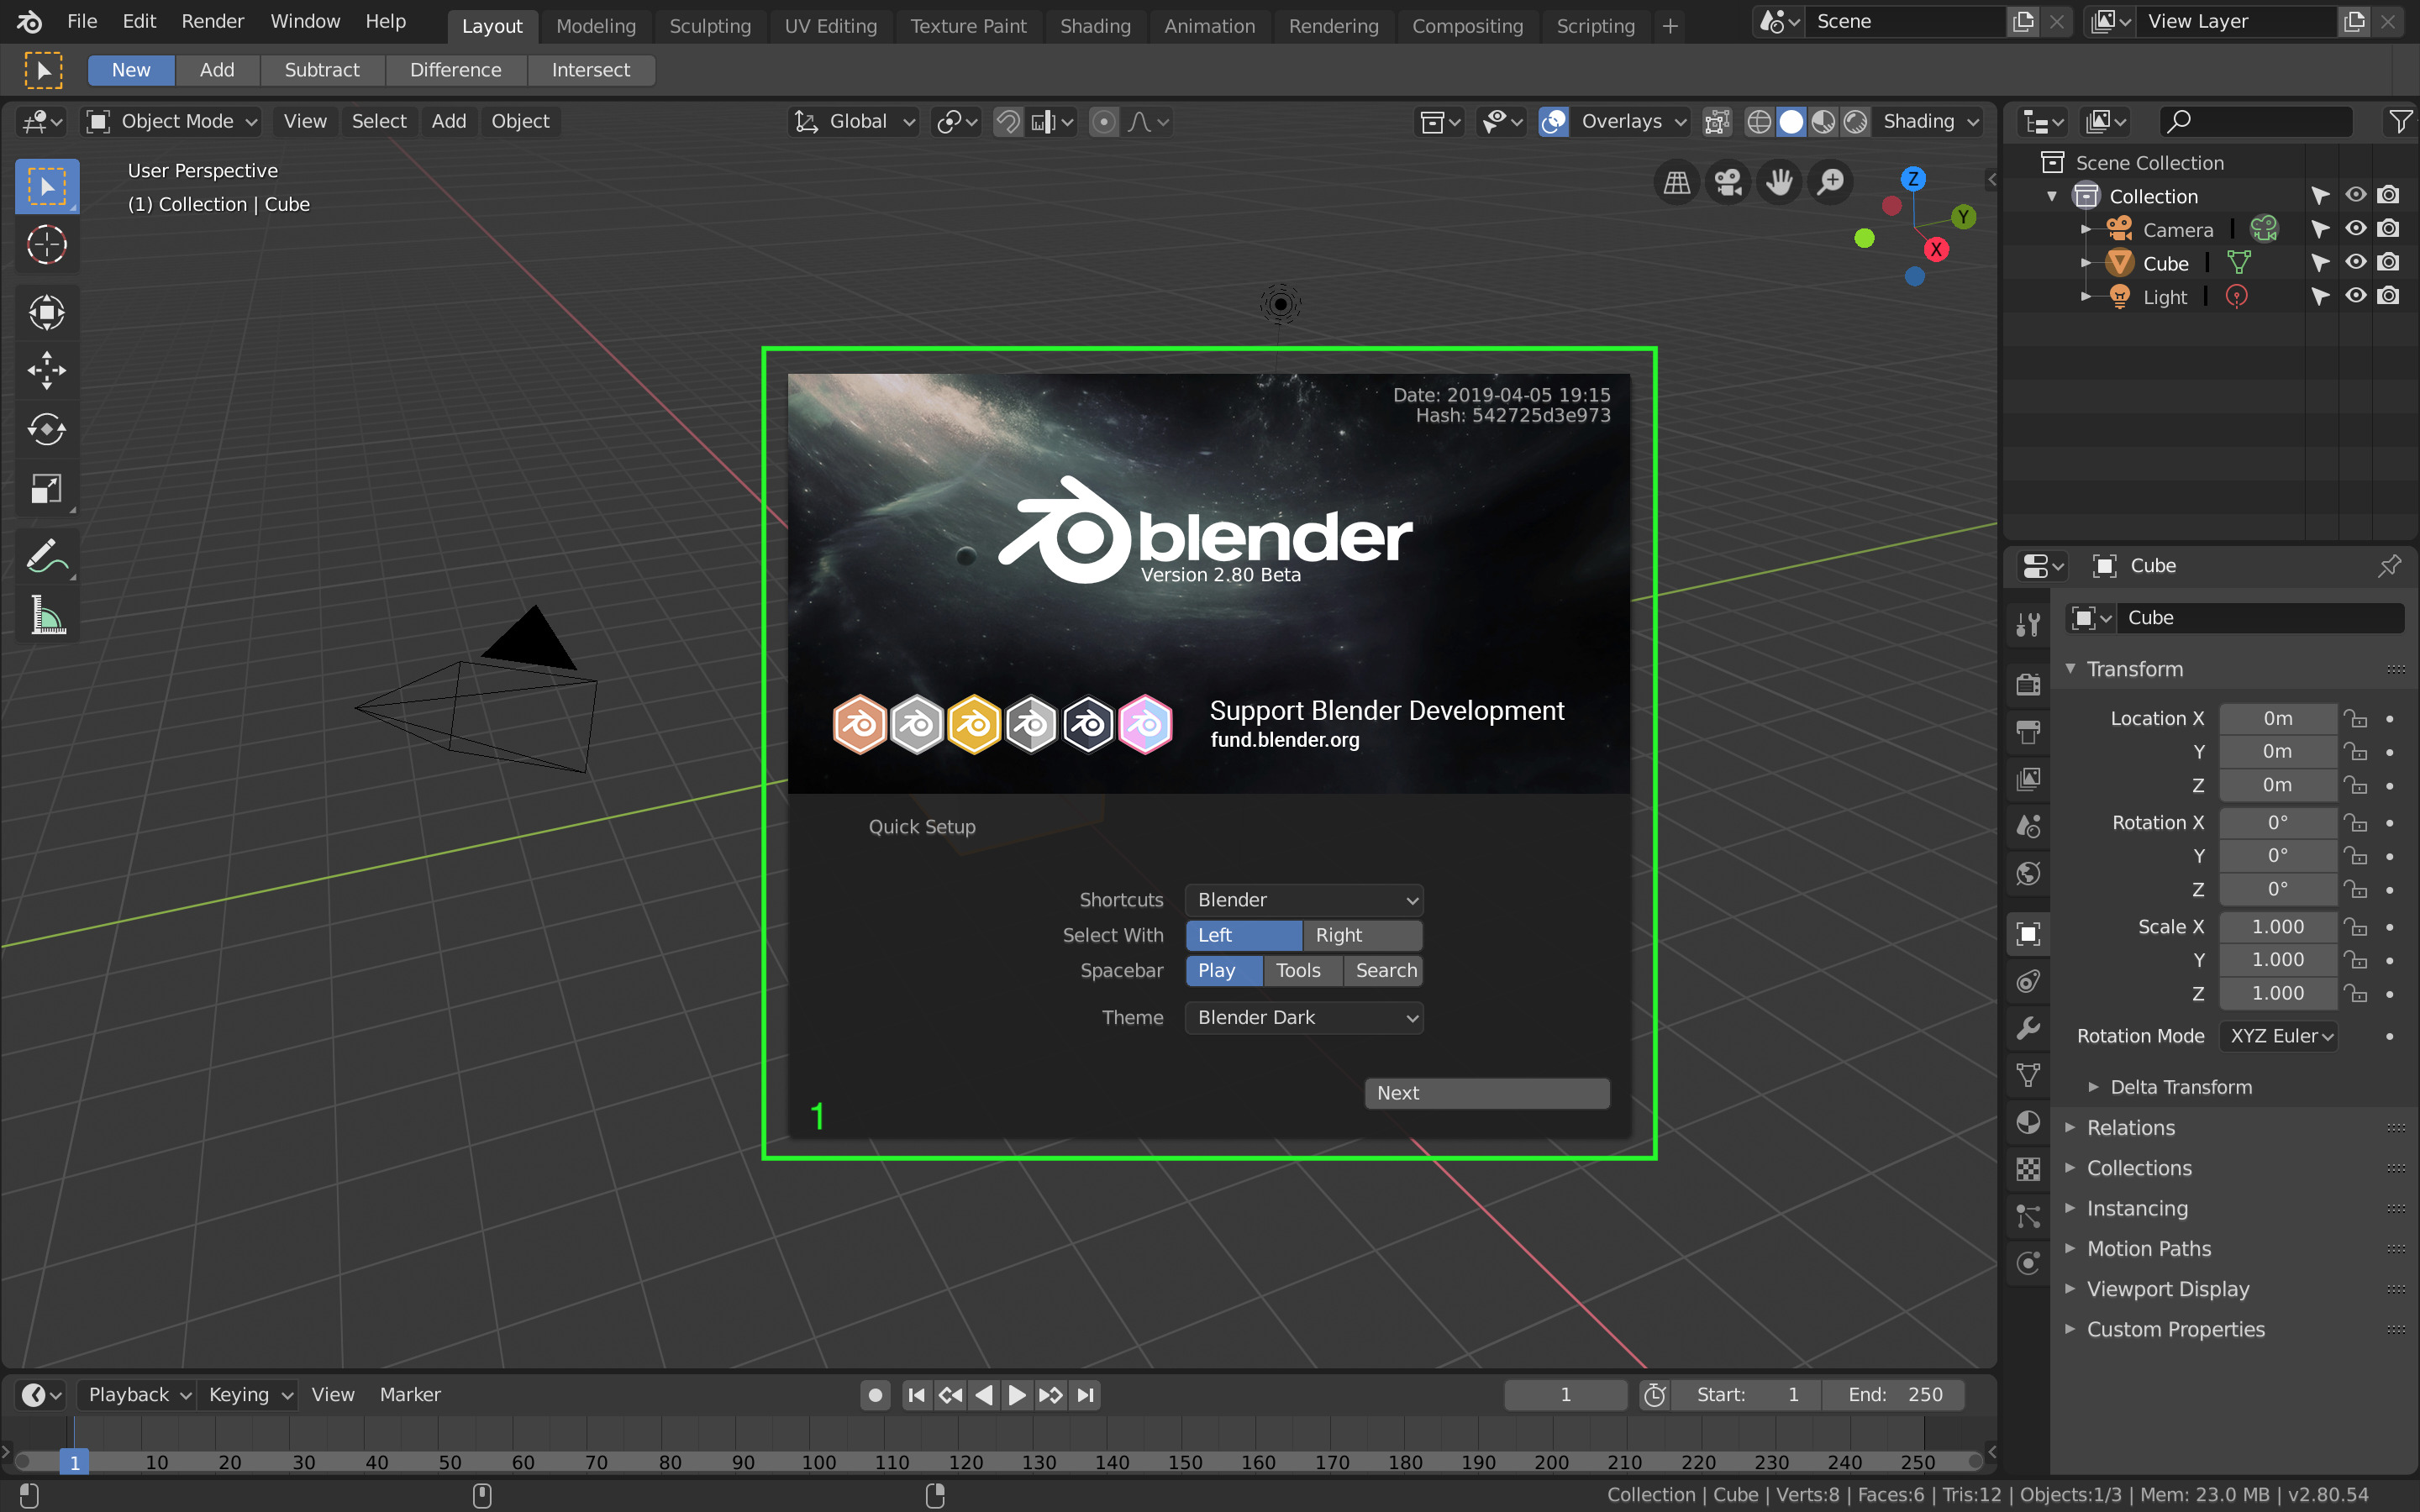
\includegraphics[width=\textwidth]{01.jpg}
        \caption{Somecaption 1}
        \label{fig:01}
    \end{minipage}
    \hfill
    \begin{minipage}[ht]{0.495\textwidth}
        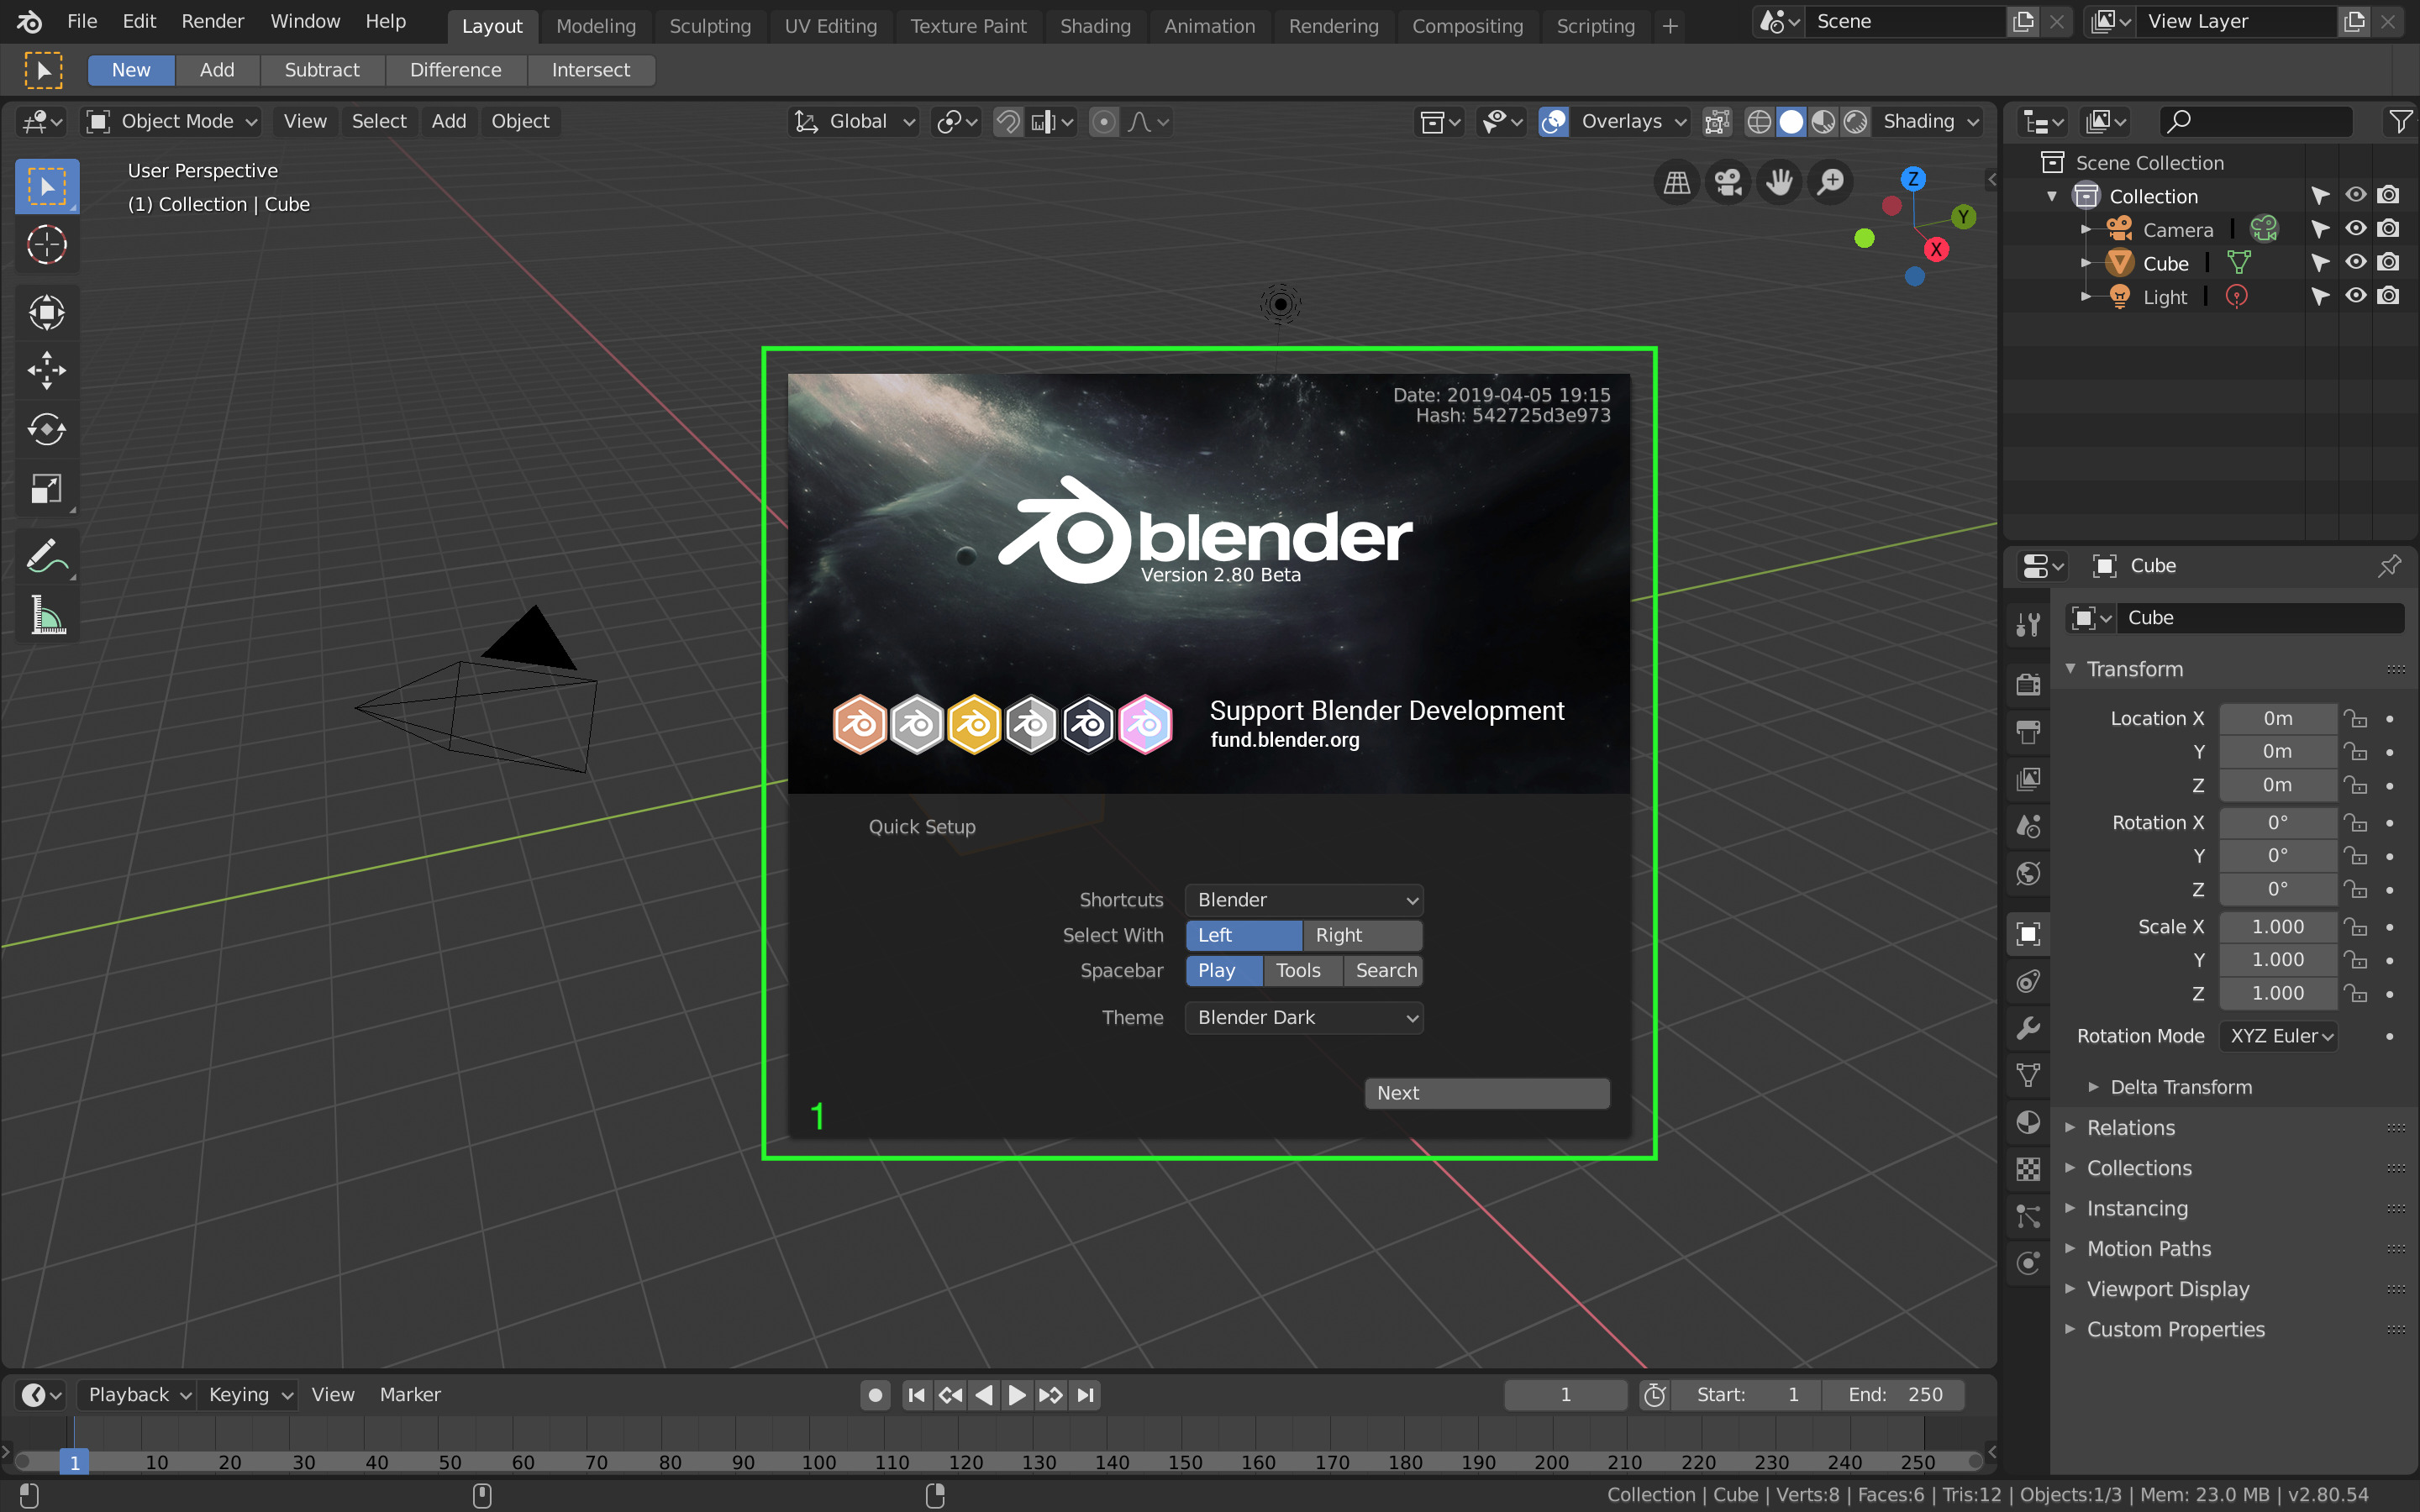
\includegraphics[width=\textwidth]{01.png}
        \caption{Somecaption 2}
        \label{fig:02}
    \end{minipage}
\end{figure}

\justify
\bibliographystyle{uts}
\bibliography{ref}
\nocite{*}

\end{document}